% ==============================================
% ELEMENTO: DESENVOLVIMENTO
% ==============================================
\section{Desenvolvimento}
\label{sec:desenvolvimento}

% ======== Dimensionamento ========
\subsection{Transistor Bias network}

O primeiro passo deste projeto foi o dimensionamento do circuito de polarização do transistor, garantindo os valores definidos
pelo professor, $I_C = 4 mA$ e $V_{CE} = 5 V$.

\begin{figure}[H]
    \centering
    \begin{subfigure}[b]{0.25\textwidth}
        \centering
        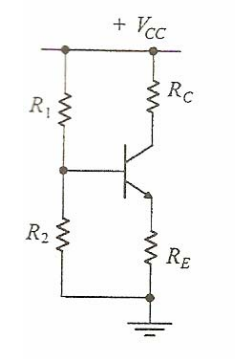
\includegraphics[width=\textwidth]{IMAGENS/LNA_antes_thevnin.png}
        \caption{Circuito inicial.}
        \label{fig:LNA_inicial}
    \end{subfigure}
    \hspace{3cm}
    \begin{subfigure}[b]{0.25\textwidth}
        \centering
        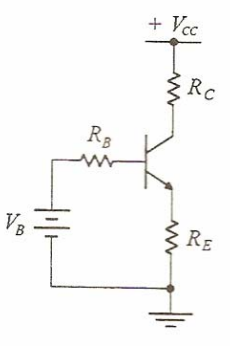
\includegraphics[width=\textwidth]{IMAGENS/LNA_depois_thevnin.png}
        \caption{Circuito após Thévenin.}
        \label{fig:LNA_depois}
    \end{subfigure}
    \caption{Circuito LNA.}
    \label{fig:LNA_comparacao}
\end{figure}

Para isso, foi utilizado o circutio da figura \ref{fig:LNA_inicial}, e depois, aplicando o teorema de Thévenin, obteve-se o circuito da figura \ref{fig:LNA_depois},
sendo este o circuito que foi utilizado para o dimensionamento, pois é mais fácil de analisar.

\begin{equation}
    V_{th} = V_{B} = V_{CC} \cdot \frac{R_2}{R_1 + R_2} \hspace{3cm} R_B = R_1 \parallel R_2
    \label{eq:thevenin}
\end{equation}


Analziando o circuito, é possível obter as seguintes expressões:
\begin{gather}
    I_B = \frac{I_C}{\beta} \hspace{1cm} I_E = I_C + I_B \hspace{1cm} V_E = I_E \cdot R_E \label{eq:correntes} \\
    R_B >> \Delta V_{BE} \hspace{1cm} V_{CC} = I_C \cdot R_C + V_{CE} + V_E \hspace{1cm} V_{th} = R_B \cdot I_B + V_{BE} + V_E \label{eq:malhas}
\end{gather}

Aqui, para facilitar as contas, assumimos que $R_B = R_E \cdot 10$, sendo um valor seguro para o circuito, pois garnate um fator de estabilidade $S$ baixo,
tornado o transistor menos sensivel a variações. Além disso,
ao invés de usar-mos o valor típico de $\Delta V_{BE}$ e assumirmos que é 0.7 V, como o transistor é de alta frequência, o valor de $V_{BE}$ é superior,
escolhendo assim 0.9 V. Ao analisar-mos o data sheet do transistor obtivemos o valor de $\beta$ para a frequência de operação,
que é de $72.532$.
Fixa-mos então apenas uma das resistências, escolhemos $R_E = 250 \Omega$, e também o valor de $V_{CC} = 10 V$, e com os valores
definidos anteriormente, $I_C = 4 mA$ e $V_{CE} = 5 V$, é possível calcular os valores das outras variáveis.


\vspace{1cm}
\begin{figure}[H]
    \centering
    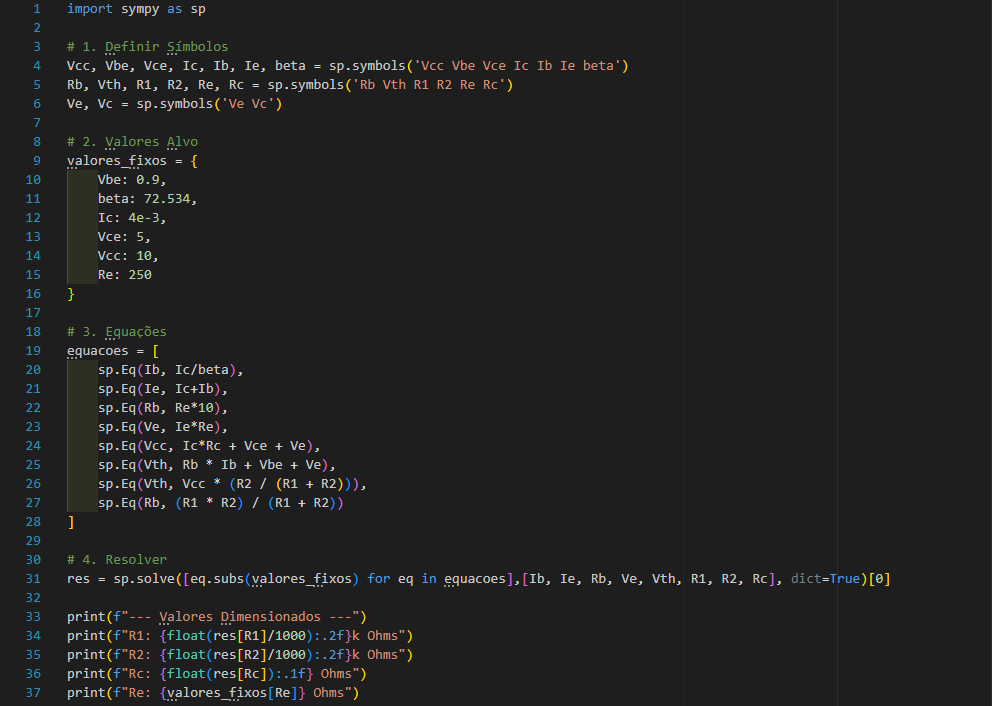
\includegraphics[width=0.7\textwidth]{IMAGENS/dimensionamento.png}
    \caption{Código usado para o dimensionamento do circuito de polarização do transistor.}
    \label{fig:sub1}
\end{figure}
\vspace{0.2cm}


Para facilitar o processo de cálculo, foi criado um código em Python, que é mostrado na figura \ref{fig:sub1}, onde apenas é necessário
introduzir os valores definidos anteriormente, e o código calcula os valores de $R_1$, $R_2$ e $R_C$ para o circuito de polarização do transistor, assim
sendo mais fácil de obtê-los e de retificar valores futuros caso necessário.

Os valores obtidos foram os seguintes: $R_1 = 12.19 k\Omega$, $R_2 = 3.15 k\Omega$ e $R_C = 996.6 \Omega$. 
Colocamos estes valores no circuito do LTspice, e simulamos o circuito para verificar se os valores de $I_C$ e $V_{CE}$ estavam corretos.
Após alguns ajustes manuais para obter os valores mais próximos possíveis dos definidos, obtivemos os seguintes valores: 
\begin{center}
    $R_1 = 9 k\Omega$ \hspace{1cm} $R_2 = 1.85 k\Omega$ \hspace{1cm} $R_C = 1.05 k\Omega$ \hspace{1cm} $R_E = 155 \Omega$
\end{center}

\vspace{1cm}
Para além do dimensionamento $DC$, a performance do LNA a $6 GHz$ depende crucialmente da introdução de componentes reativos, que desempenham funções distintas.
Assim, foram adicionadas primeiramente bobinas em série tanto na base como no coletor. Como o circuito é Emissor-Comum, o sinal $V_{IN}$ encontra-se
na base e a saída no coletor.

Estas bobinas são importantes, pois em $DC$ funcionam como Curto-Circuito, não influenciando o circuito, mas em $AC$ possuem
uma impedância muito elevada ($Z_L = j \cdot \omega \cdot L$). Esta característica faz com que o sinal seja "forçado"
a entrar no trasnsístor, impedindo que o sinal em altas frequências seja "curto-circuitado" pela fonte de alimentação
ou dissipado nas resistências de polarização.

Já os condensadores foram adicionados tanto na base e no coletor, em série, mas também no emissor, sendo neste em paralelo. Estes desempanham a função
contrária às bobinas, pois ao invés de deixarem passar sinal $DC$ e bloquearem $AC$, fazem o inverso, bloqueiam o sinal em $DC$ enquanto
em $AC$ permitem o sinal passar.

analisarNo emissor, o condensador tem como função efetuar um bypass de RF (Radiofrequência), ou seja, como a impedância do condensador é muito baixa ($Z_C = \frac{1}{j \cdot \omega \cdot C}$),
o sinal esolhe o caminho com menor impedância, logo em $AC$ o sinal irá estar diretamente ligado à massa, em quanto em $DC$ será circuito aberto.
Na base e no coletor eles servem para bloquear os sinais $DC$. Como dito anteriormente, em $DC$ um condensador será equivalente a um
circuito aberto, e assim em $AC$ deixa passar o sinal e impede que haja uma tensão $DC$.

Desta forma, os condensadores na base e no coletor atuam como elementos de acoplamento,
removendo qualquer offset de tensão contínua. Na base, isto impede que a polarização do transístor
seja afetada pela fonte de sinal; no coletor, garante que a carga de $50\ \Omega$ receba apenas o sinal de
RF amplificado, sem a componente $V_{CC}$.


% ======== LTspice ========
\subsection{Implementação em LTspice e obtenção dos parâmetros S do transistor}

\begin{figure}[H]
    \centering
    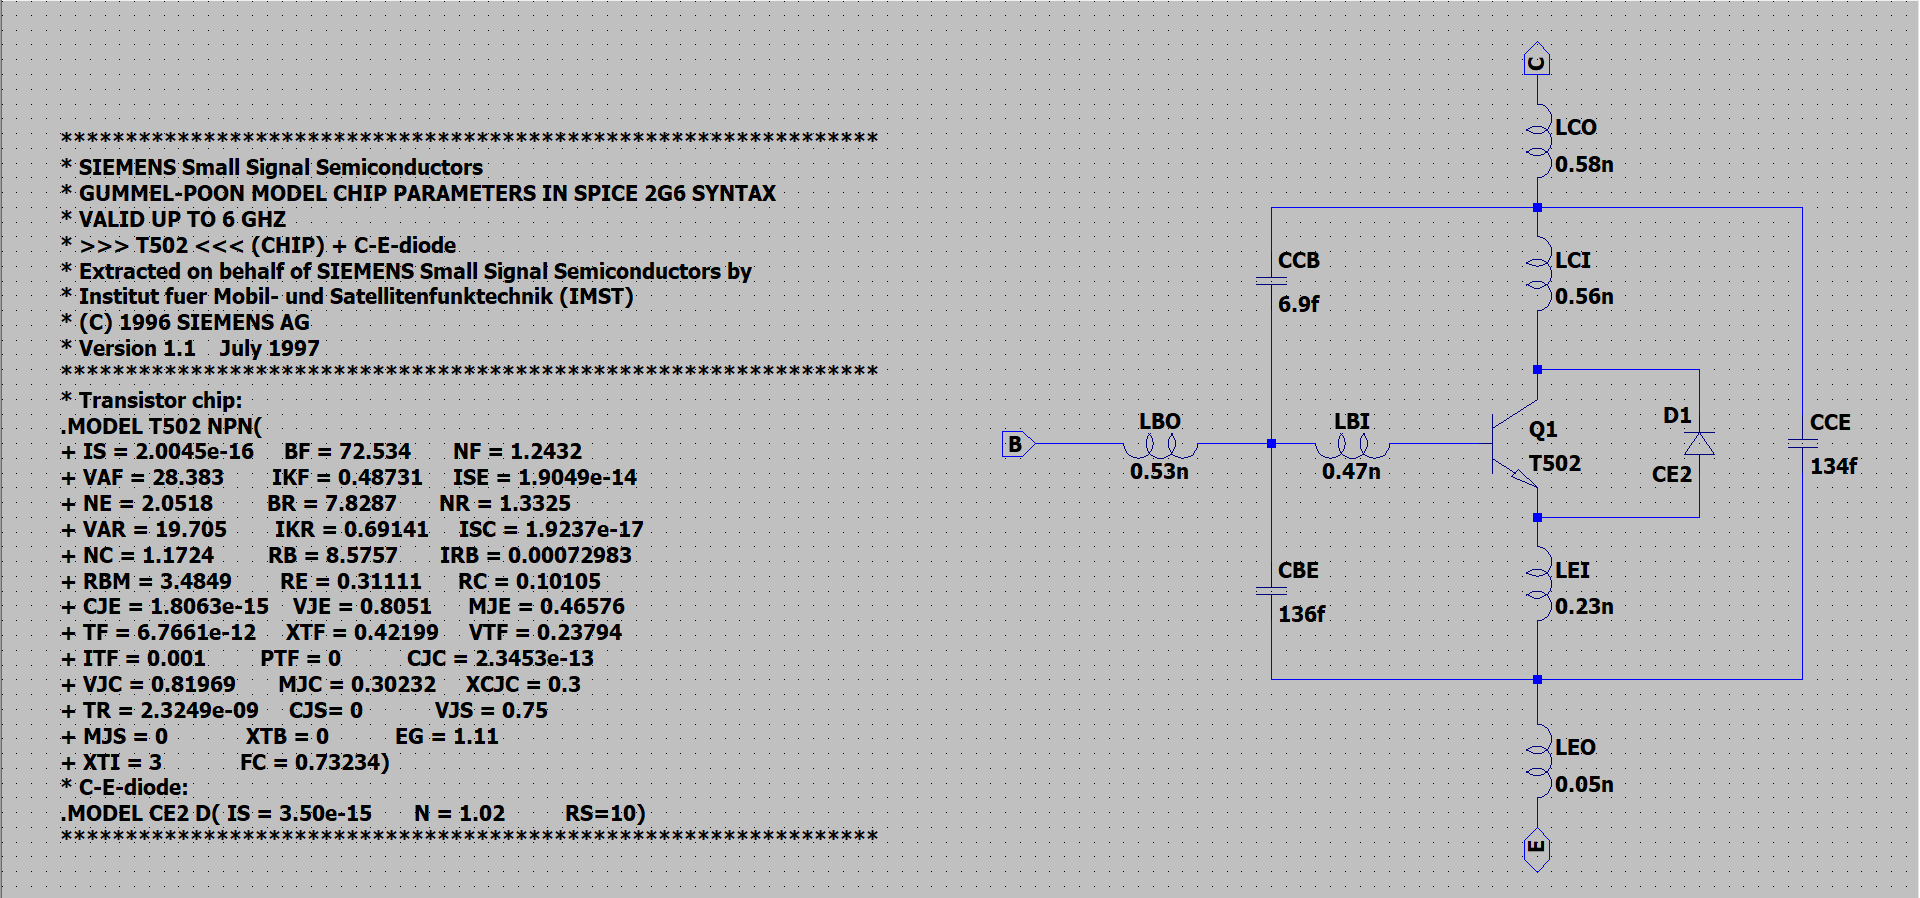
\includegraphics[width=0.9\textwidth]{IMAGENS/transistor_ltspice.png}
    \caption{Circuito do transistor BFP420 em LTspice.}
    \label{fig:LNA_inicial}
\end{figure}
\vspace{0.2cm}

\begin{figure}[H]
    \centering
    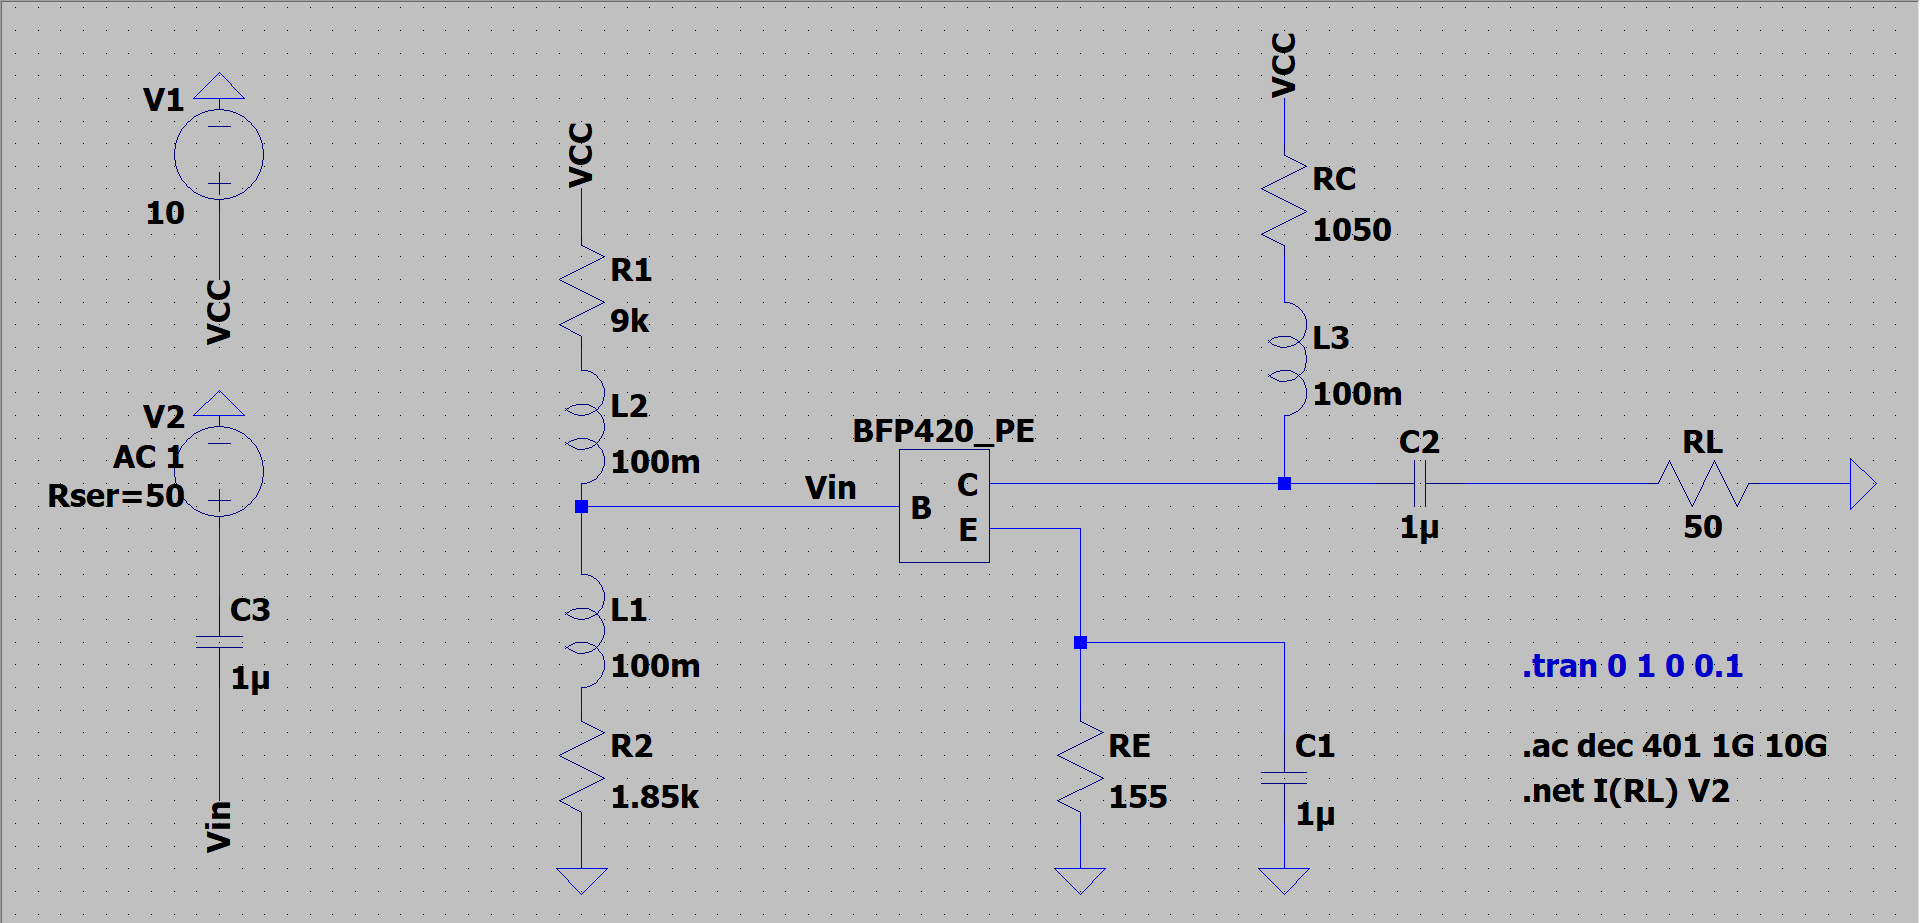
\includegraphics[width=0.9\textwidth]{IMAGENS/LNA_LTspice.png}
    \caption{Circuito simulado no LTspice.}
    \label{fig:lna_ltspice}
\end{figure}
\vspace{0.2cm}

\begin{figure}[H]
    \centering
    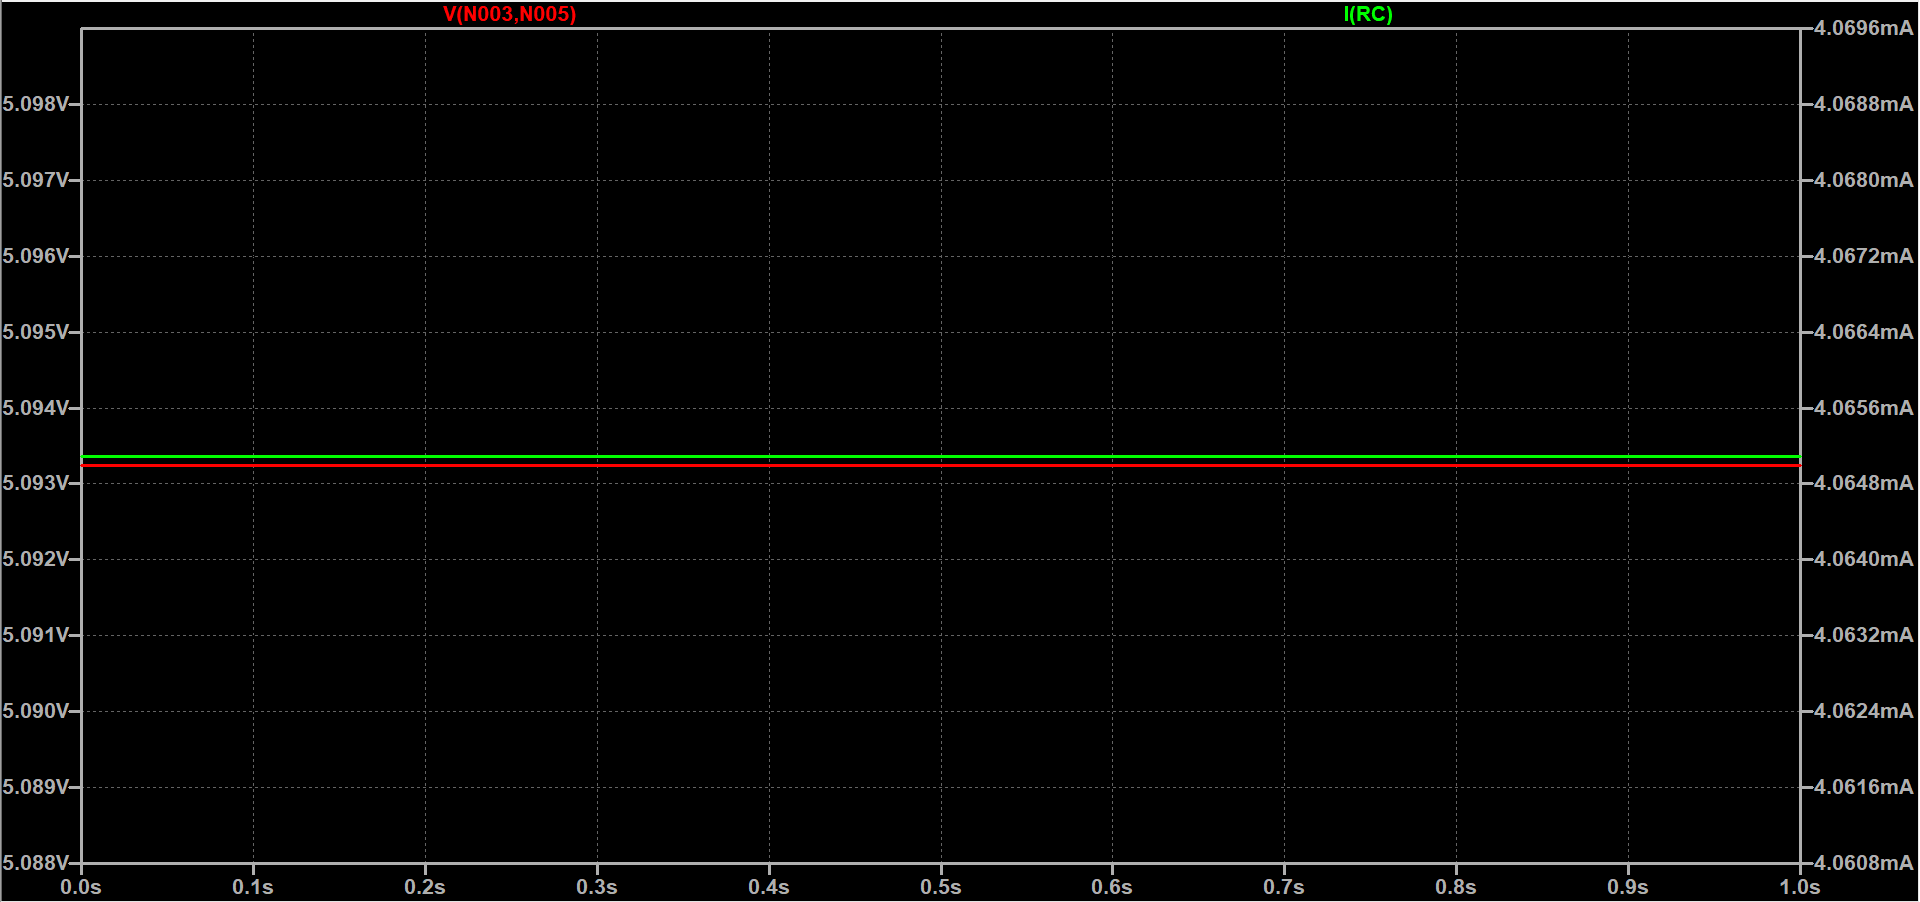
\includegraphics[width=0.9\textwidth]{IMAGENS/dimensionamento_ltspice.png}
    \caption{Circuito simulado no LTspice.}
    \label{fig:dimensionamento_ltspice}
\end{figure}
\vspace{0.2cm}

Assim, confirmamos o valor de $I_C = 4.065 mA$ e $V_{CE} = 5.093 V$, o que é muito próximo dos valores
definidos inicialmente, e portanto, o circuito de polarização do transistor está dimensionado corretamente.

Assim prosseguimos para a obtenção dos parâmetros S do transistor, que são essenciais para o projeto do LNA, e que serão utilizados posteriormente para a análise de estabilidade e adaptação do circuito.

\begin{figure}[H]
    \centering
    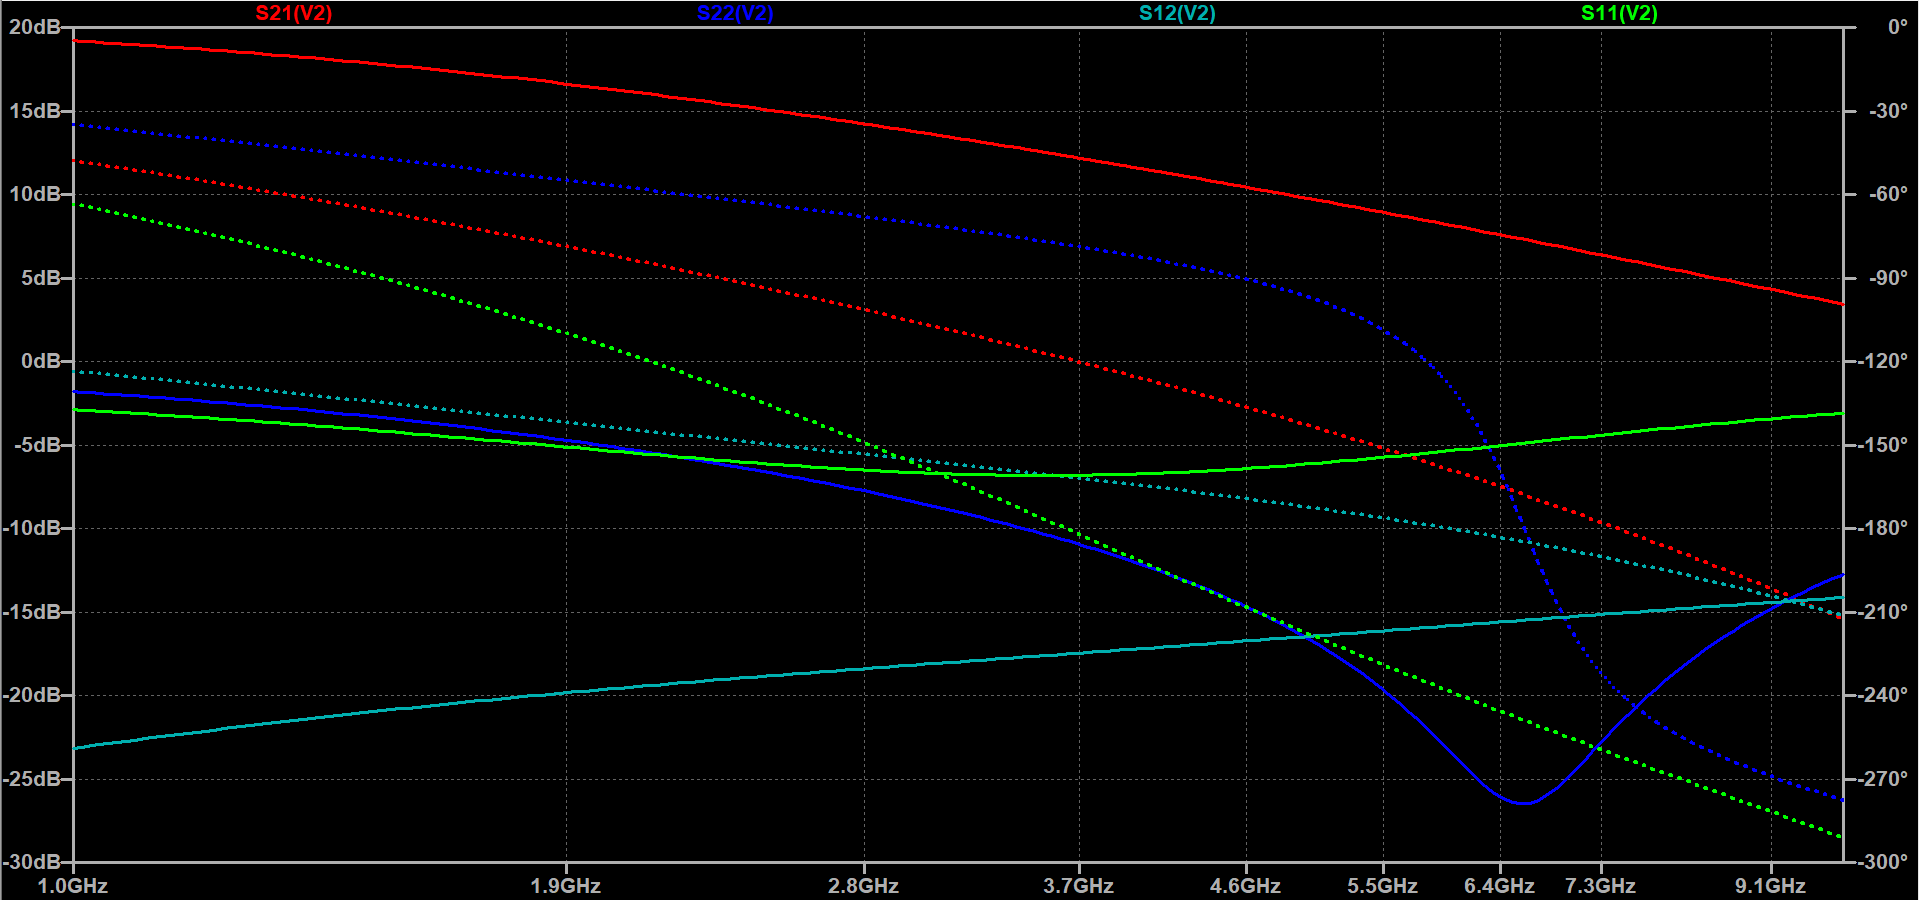
\includegraphics[width=0.9\textwidth]{IMAGENS/S_ltspice.png}
    \caption{Parâmetros S do transistor no LTspice.}
    \label{fig:parametros_s_ltspice}
\end{figure}
\vspace{0.2cm}

Através desta análise, extraíram-se os parâmetros $S$ do transístor para o intervalo de $1\text{ GHz}$ a $10\text{ GHz}$.
Foi aplicado um varrimento com passo de $0,5\text{ GHz}$, tendo-se aumentado a resolução para passos
de $0,25\text{ GHz}$ no intervalo entre $3\text{ GHz}$ e $6\text{ GHz}$. Esta densidade de dados superior
na zona de operação pretendida é fundamental para garantir a precisão nos cálculos posteriores de
estabilidade e de adaptação de impedâncias.

A extração dos parâmetros foi realizada recorrendo à diretiva $.net$, definindo a porta de entrada 
a base e a carga no coletor, permitindo obter os S-parameters necessários para validar o ganho ($S_{21}$)
e as reflexões $S_{11} e S_{22}$.

% ======== AppCAD ========
\subsection{Análise dos coeficientes de reflexão em AppCAD}

\begin{figure}[H]
    \centering
    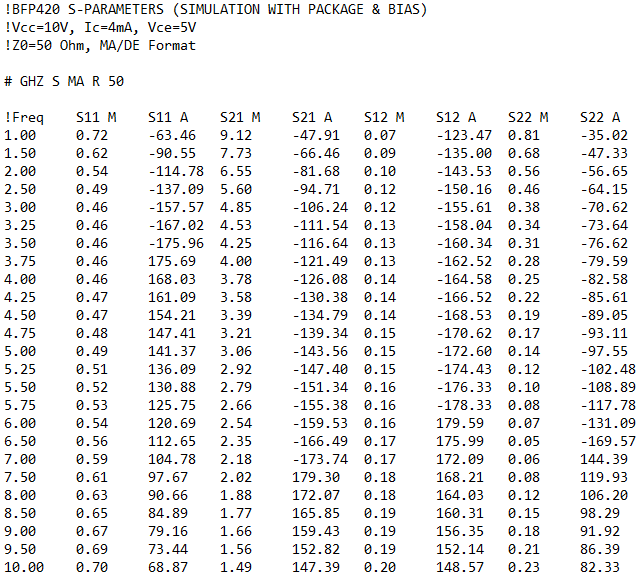
\includegraphics[width=0.7\textwidth]{IMAGENS/ficheiro_s2p.png}
    \caption{Valores dos parâmetros S para as frequências de 1 GHz a 10 GHz.}
    \label{fig:ficheiro_s2p}
\end{figure}
\vspace{0.2cm}

Com estes valores o próximo passo foi introduzir estes dados no software AppCAD, para obter os coeficientes de reflexão simultaneamente adaptados ($\Gamma_{MS}$ e $\Gamma_{ML}$), garantindo a estabilidade e o ganho pretendido.
Para isso, foi necessário criar um ficheiro .s2p com os valores dos parâmetros S (figura \ref{fig:ficheiro_s2p}), e depois analisar para que valores de frequência o circuito era estável.

\begin{figure}[H]
    \centering
    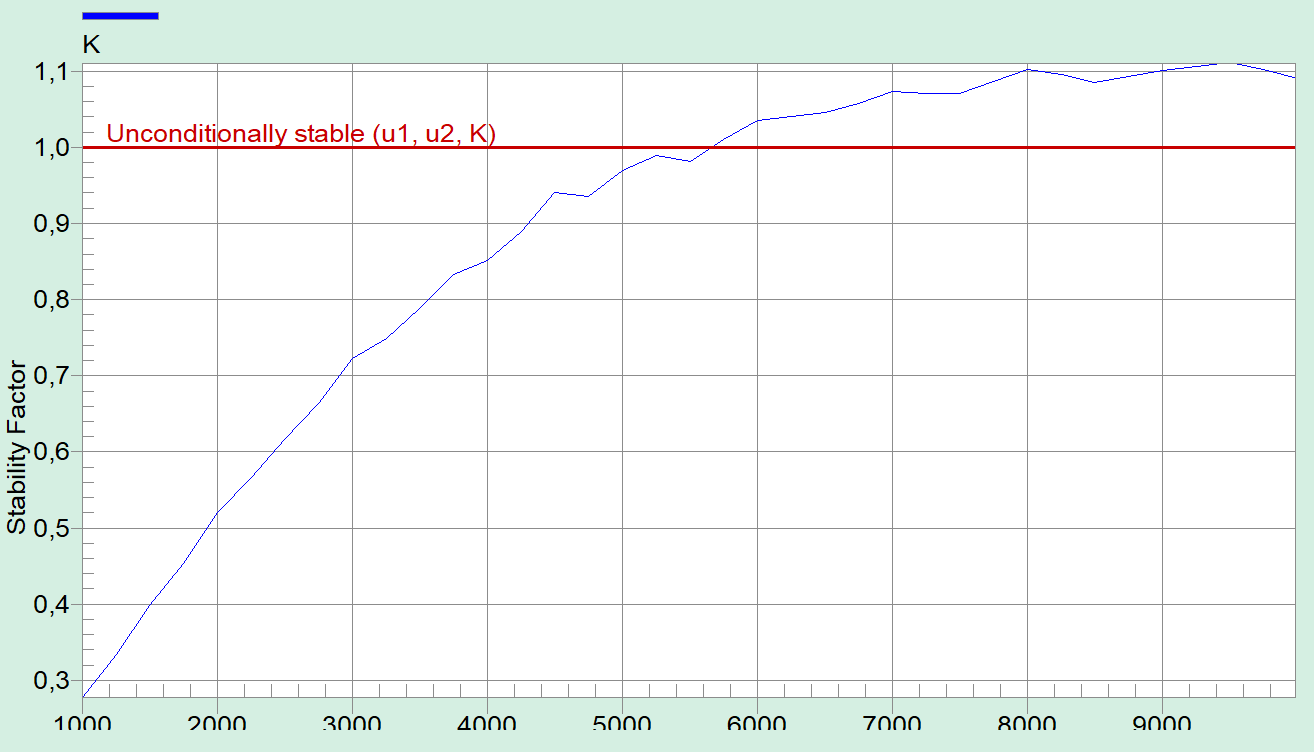
\includegraphics[width=0.7\textwidth]{IMAGENS/k_appcad.png}
    \caption{Valor de K para as frequências de 1 GHz a 10 GHz.}
    \label{fig:valores_estabilidade_k}
\end{figure}
\vspace{0.2cm}

Com a figura \ref{fig:valores_estabilidade_k} é possível verificar que o circuito é estável para frequências
superiores a $5.5 GHz$, e portanto, a frequência de operação escolhida para o projeto do LNA foi de $6 GHz$.

Este valor de frequência é bastante próximo do limite superior do transistor, e portanto, foi ponderada a troca
da corrennte de polarização $I_C$ para $7 mA$ ao invés dos $4 mA$. O aumento desta corrente permite que
o transistor tenha um valor de $k > 1$ em frequências mais baixas, comparado com o valor usado.
Isto acontece pois a transcondutância do transistor é diretamente proporcional à corrente no coletor, assim fazendo que
ao aumentar essa corrente o trnasistor tenha uma maior amplificação.

Contudo, $6 GHz$ apesar de estar no limite ainda está dentro da gama de valores de frequência que o transistor aguenta,
por isso decidiu manter-se os valores atuais.


\begin{figure}[H]
    \centering
    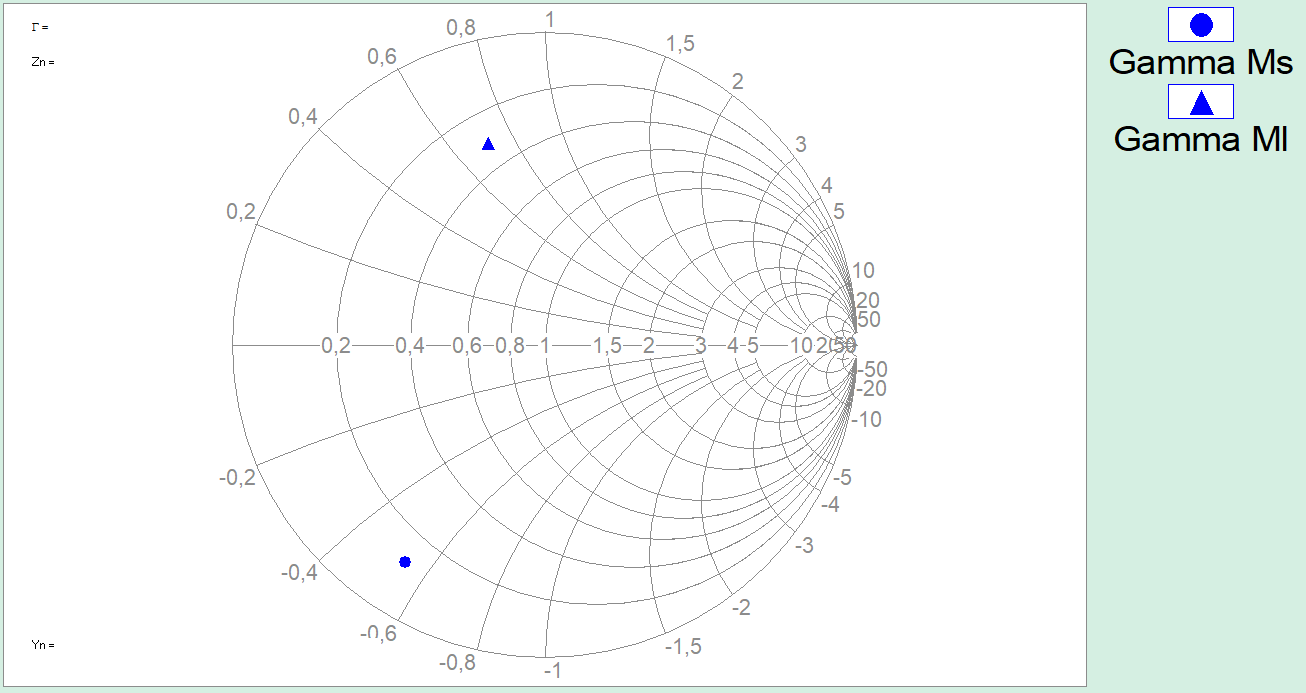
\includegraphics[width=0.7\textwidth]{IMAGENS/gamma_appcad.png}
    \caption{Coeficientes de reflexão para $F = 6GHz$.}
    \label{fig:valores_estabilidade_k}
\end{figure}
\vspace{0.2cm}

Com a frequência atribuida, o próximo passo era retirar os valores dos coeficientes de reflexão da
entrada e da saída, $\Gamma_{MS}$ e $\Gamma_{ML}$, respetivamente.

Podemos observar pela figura \ref{fig:valores_estabilidade_k} que os valores são, em impedância $Z_{S}$ e $Z_{L}$:
\begin{center}
    $Z_{S} = 0.33 +j0.70$ \hspace{1cm} $Z_{L} = 0.12 - j0.54$
\end{center}

\vspace{0.5cm}
Estes valores já se encontram normalizados à impednância característica da linha, $Z = 50 \Omega$.



% ======== LTspice adaptação ========
\subsection{Adaptação do circuito no LTspice}

O próximo passo era realizar a adaptação do circuito usando a Carta de smith.

% ======== LTspice adaptação: C & B ========
\subsubsection{Adaptação do circuito no LTspice usando Condensadores e Bobinas}

A primeira adaptação a ser feita foi com Condensadores e bobinas.

\begin{figure}[H]
    \centering
    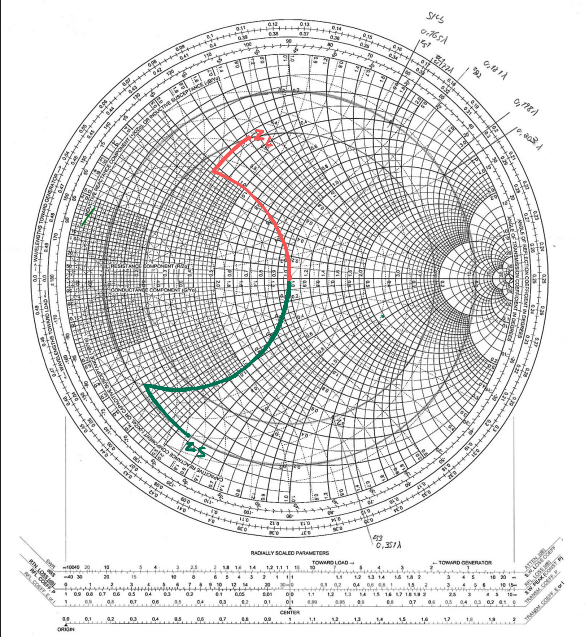
\includegraphics[width=0.7\textwidth]{IMAGENS/CS_CB.png}
    \caption{Carta de Smith para Condensadores e Bobinas}
    \label{fig:carta_smith}
\end{figure}

\textbf{Adaptação de Entrada ($Z_{S}$):}

Para $Z_S$, partindo da origem ($Z_C = 1 + j0$), seguimos até ao ponto $Z_{aux} = 0.12 - j0.32$ pela
circunferência de admitância no sentido horário (adicionando suscetância positiva), o que corresponde a um
condensador em paralelo. Desse ponto, seguimos pela circunferência de impedância ($Re = 0.12$) no sentido
anti-horário (adicionando reatância negativa) até atingir $Z_S = 0.12 - j0.54$, o que corresponde a um
condensador em série.

Calculando o condensador em paralelo ($\Delta b = j2.74$):
\begin{center}
    $Y_{aux} = \frac{1}{0.12 - j0.32} \approx 1 + j2.74$ \hspace{1cm} $C_p = \frac{2.74}{\omega \cdot Z_0} \approx 1.45\,pF$
\end{center}

Para o condensador em série, calculamos a diferença de reatância:
\begin{center}
    $\Delta x = \text{Im}(Z_S) - \text{Im}(Z_{aux}) = -0.54 - (-0.32) = -0.22$
\end{center}
Usando a expressão $C_s = \frac{1}{0.22 \cdot \omega \cdot Z_0}$, obtemos $C_s \approx 2.41\,pF$.

\vspace{0.5cm}
\textbf{Adaptação de Saída ($Z_{L}$):}

Para $Z_L$, o primeiro passo foi partir do centro da carta ($Z_{C} = 1 + j0$). Deste ponto seguimos pela
circunferência de admitância ($Re = 1$) no sentido anti-horário até chegar ao ponto auxiliar
$Z_{aux} = 0.33 + j0.47$, o que corresponde à introdução de uma bobina em paralelo. 
De seguida, avançou-se pela circunferência de impedância ($Re = 0.33$) no sentido horário até ao ponto
de carga ótima $Z_{L} = 0.33 + j0.70$, o que equivale a adicionar uma bobina em série.

Assim, calculamos a bobina em paralelo através das admitâncias:
\begin{center}
    $Y_C = 1 + j0$ \hspace{1cm} $Y_{aux} = \frac{1}{0.33 + j0.47} \approx 1 - j1.43$
\end{center}
Com $\Delta b = -j1.43$, obtemos $L_p = \frac{Z_0}{1.43 \cdot \omega} \approx 0.93\,nH$.

Para a bobina em série, subtraímos as impedâncias: $\Delta x = Z_L - Z_{aux} = j0.70 - j0.47 = j0.23$.
Obtemos $L_s = \frac{Z_0 \cdot 0.23}{\omega} \approx 0.305\,nH$.

\vspace{1cm}
\textbf{Adaptação em LTspice:}

Com os valores calculados, procedeu-se à implementação no LTspice para validar a adaptação.
Na rede de entrada (fonte), foram adicionados os dois condensadores calculados ($C_p = 1.45\,pF$ e $C_s = 2.41\,pF$)
antes do condensador de bloqueio $C_3$. Na rede de saída (carga), foram colocadas as bobinas
($L_p = 0.93\,nH$ e $L_s = 0.305\,nH$) após o condensador de bloqueio $C_2$. 

Esta disposição garante que os componentes de adaptação não interferem com a polarização DC do
transístor, mantendo o ponto de operação estável enquanto realizam a transformação de impedância para
$50\,\Omega$ na frequência de $6\,GHz$.


\begin{figure}[H]
    \centering
    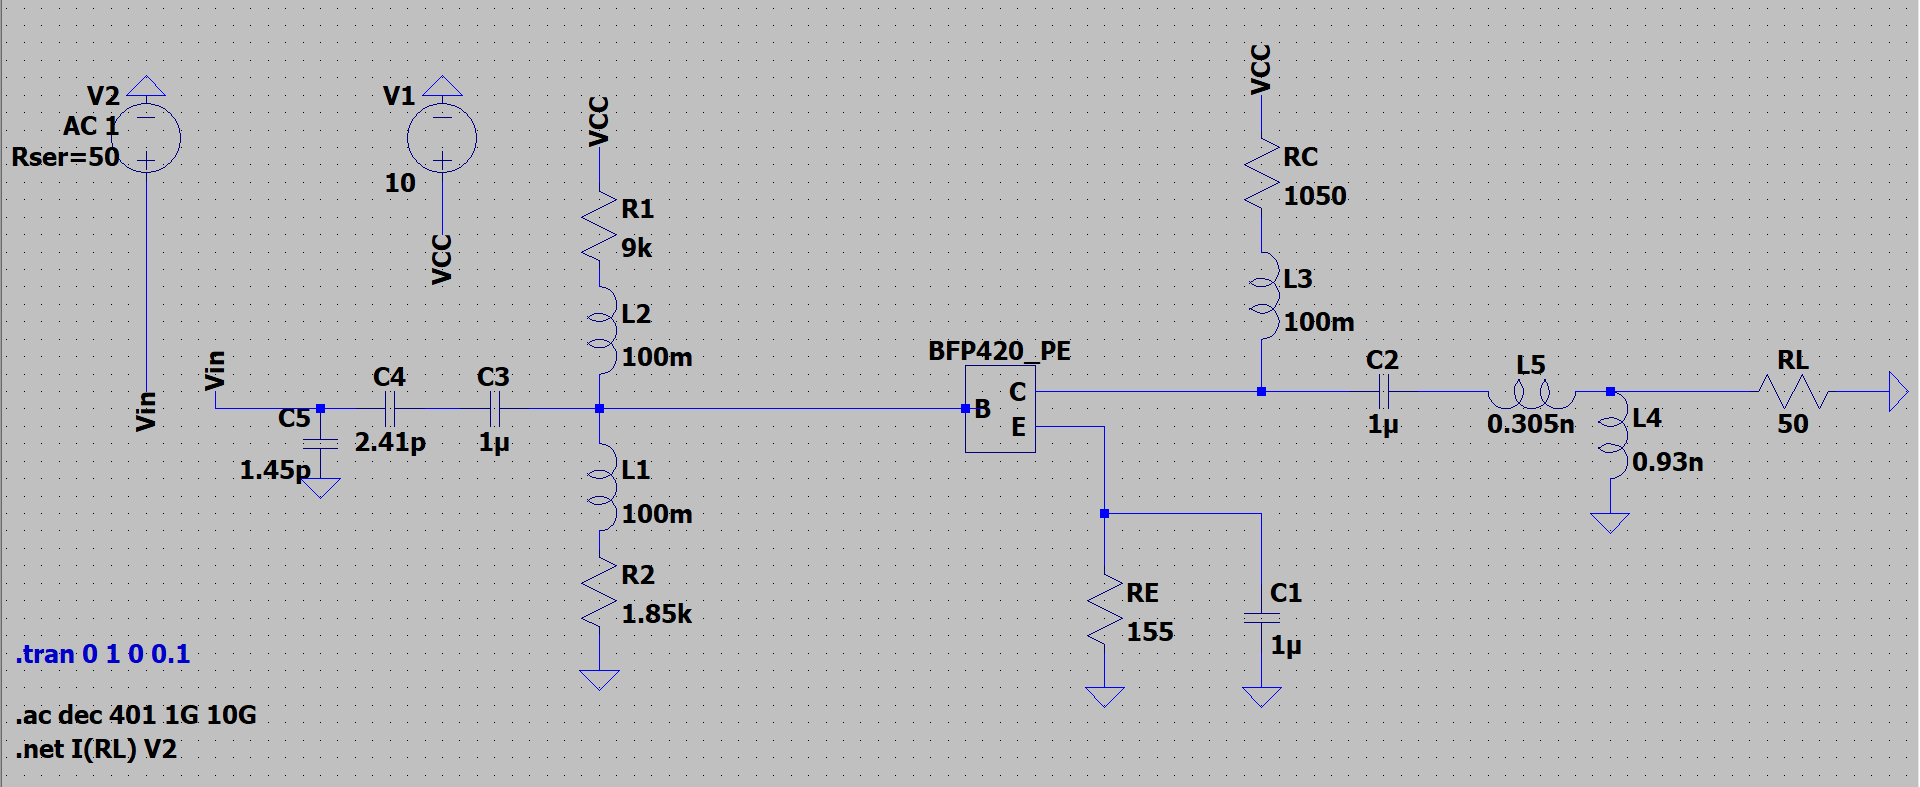
\includegraphics[width=0.8\textwidth]{IMAGENS/ltspice_CB.png}
    \caption{Circuito adaptado com Condensadores e Bobinas}
    \label{fig:LTspice_CB_circuito}
\end{figure}

\begin{figure}[H]
    \centering
    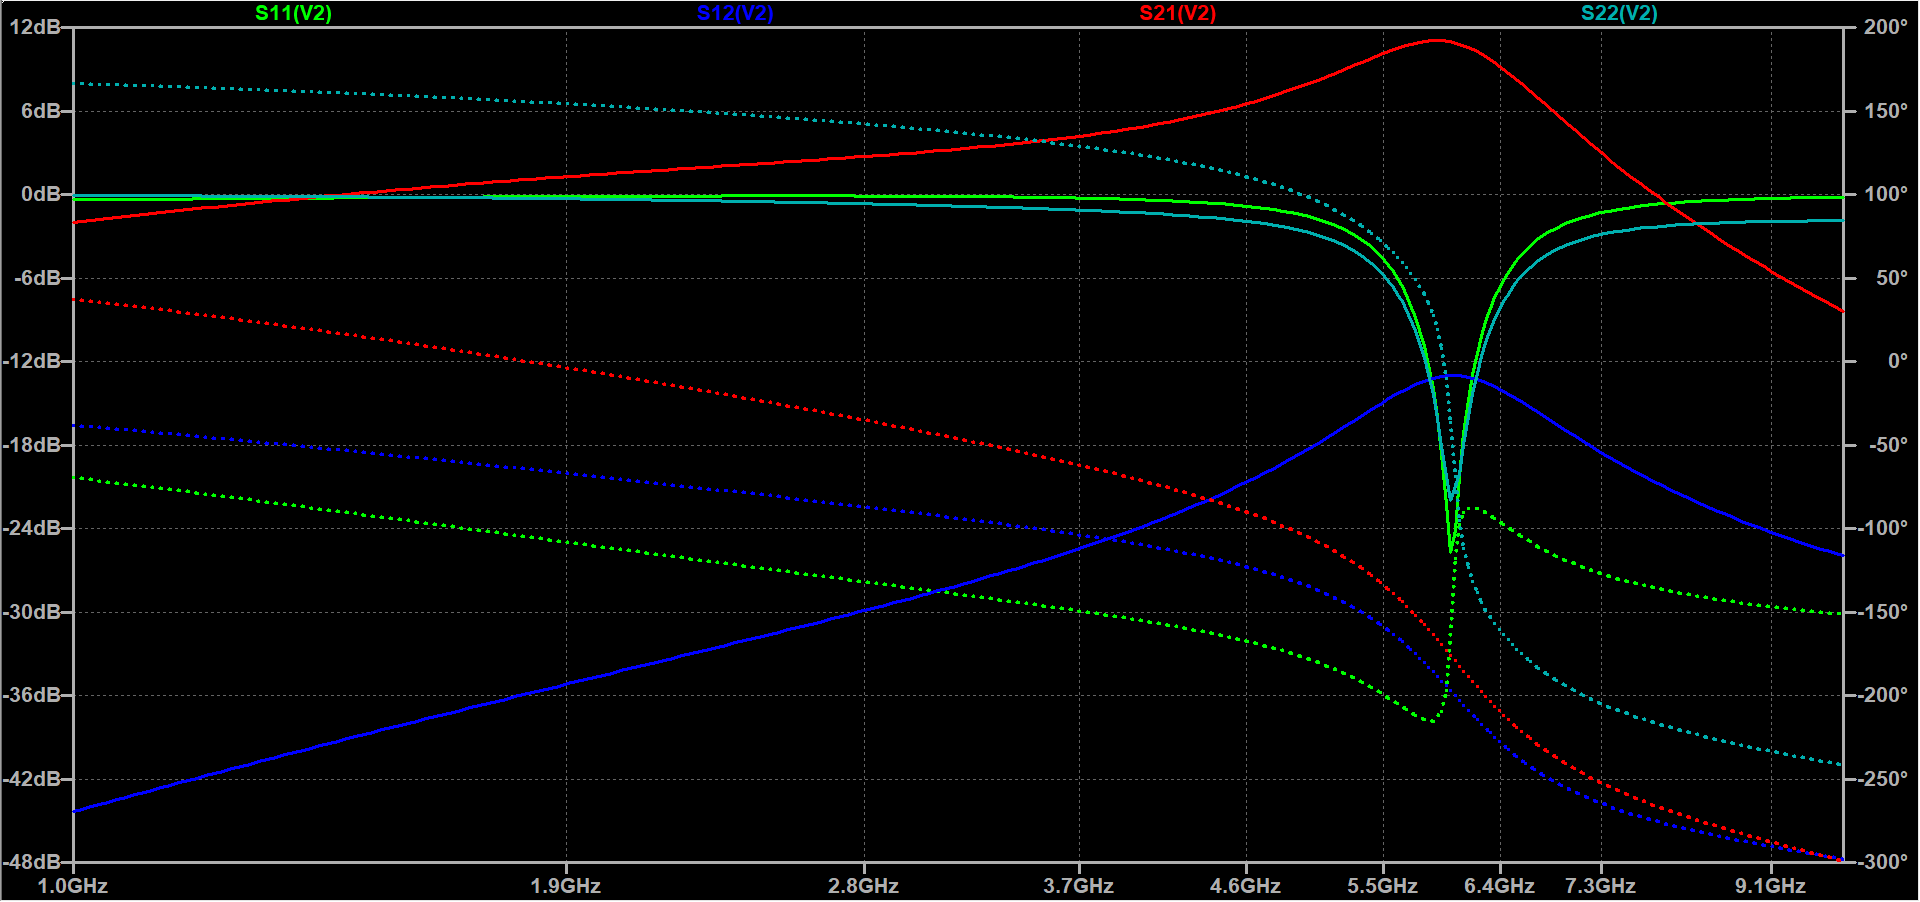
\includegraphics[width=0.8\textwidth]{IMAGENS/ltspice_CB_s.png}
    \caption{Parâmetros S do circuito adaptado com Condensadores e Bobinas}
    \label{fig:LTspice_CB_s}
\end{figure}

\vspace{0.5cm}
\begin{figure}[htbp]
    \centering
    \begin{subfigure}[b]{0.32\textwidth}
        \centering
        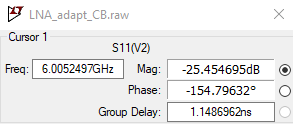
\includegraphics[width=\textwidth]{IMAGENS/ltspice_CB_S11.png}
        \caption{Parâmetro $S_{11}$ (Entrada).}
        \label{fig:s11_cb}
    \end{subfigure}
    \hfill
    \begin{subfigure}[b]{0.32\textwidth}
        \centering
        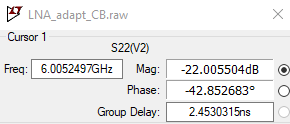
\includegraphics[width=\textwidth]{IMAGENS/ltspice_CB_S22.png}
        \caption{Parâmetro $S_{22}$ (Saída).}
        \label{fig:s22_cb}
    \end{subfigure}
    \hfill
    \begin{subfigure}[b]{0.32\textwidth}
        \centering
        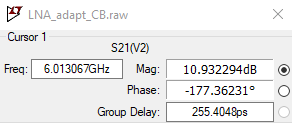
\includegraphics[width=\textwidth]{IMAGENS/ltspice_CB_S21.png}
        \caption{Parâmetro $S_{21}$ (Ganho).}
        \label{fig:s21_cb}
    \end{subfigure}

    \caption{Valores dos parâmetros S do circuito adaptado com Condensadores e Bobinas}
    \label{fig:valores_s_cb_ltspice}
\end{figure}

\vspace{1cm}
Através das figuras \ref{fig:LTspice_CB_s} e \ref{fig:valores_s_cb_ltspice} conseguimos confirmar a adaptação calculada
anteriormente. Como podemos observar, na frequência escolhida, $f = 6~GHz$, temos os valores do parâmetro de entrada e de saída,
$S_{11}$ e $S_{22}$ inferiores aos $-10~dB$, sendo estes $-25.45~dB$ e $-22.01~dB$ respetivamente, e o valor do ganho $S_{21} = 10.93~dB$, que é um valor
considerado bom para o LNA.


% ======== LTspice adaptação: L & S ========
\vspace{1cm}
\subsubsection{Adaptação do circuito no LTspice usando Linhas e Stubs}

Para a adaptação com linhas de transmissão, utilizou-se a técnica de stub simples em paralelo e circuito aberto e uma linha em série.

O processo iniciou-se com a conversão das impedâncias $Z_S$ e $Z_L$ para as suas admitâncias equivalentes $Y_S$ e $Y_L$,
facilitando o cálculo de elementos em paralelo. Iremos então guardar os valores dos pontos, e como estamos em admitância
foram lidos na linha que cruza em $Wavelengths~Toward~Generator$.

Para calcular o valor da linha seguimos pelo sentido anti-horário (pois estamos em admitânica, logo corresponde ao sentido comprimentos de onda em direção ao gerador)
da circunferência com centro em $Z_C = 1+j0$ e de raio o valor do centro até ao ponto de admitância obtido, ou seja ROE constante, até chegar
ao ponto onde intersecta a circunferência de impedância com parte real positiva $RE = 1$, circunferência de condutância unitária ($g = 1$).
A diferença entre os valores lidos na escala de comprimentos de onda entre estes dois pontos determina o comprimento elétrico da linha em série em função de $\lambda$

Para calcular o stub, no ponto de interseção a admitância possui uma componente imaginária (suscetância). O comprimento do stub em
circuito aberto é determinado pela distância necessária na Carta de Smith até a essa componente imaginária.

Depois, para adicionar no LTspice apenas é necessário calcular o atraso da linha, sendo a expressão:

\begin{center}
    $T_d = \frac{\text{Wavelength (em }\lambda\text{)}}{\text{frequência}}$
\end{center}


% ======== LTspice adaptação: L & S - ZS ========
\newpage
\textbf{Adaptação de Entrada \texorpdfstring{$Z_{S}$}{ZS}}
\begin{figure}[H]
    \centering
    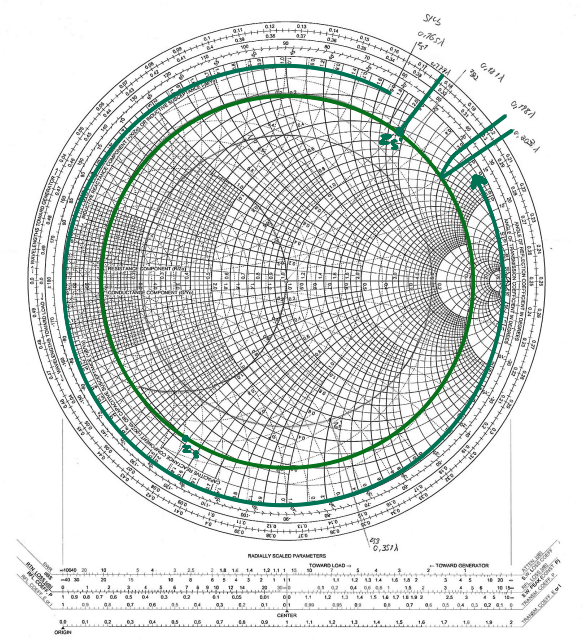
\includegraphics[width=0.65\textwidth]{IMAGENS/CS_LS_ZS.png}
    \caption{Carta de Smith para Linhas e Stubs, $Z_{S}$}
    \label{fig:carta_smith_ls_zs}
\end{figure}


Primeiro vamos adaptar a impedãncia de entrada $Z_S = 0.12-j0.54$

Assim, passamos o valor para admitânica e obtemos o valor $Y_S = 0.39 + j1.76$ com o comprimento
de onda em direção ao gerador de $\lambda_{L1} = 0.177~\lambda$

Assim, seguindo até ao ponto de interseção, o valor obtido é $\lambda_{L2} = 0.203~\lambda$. Como seguimos pelo sentido
anti-horário e passamos pelo $0~\lambda$ na cartam, o valor a colocar na linha é:
\begin{center}
    $0.500\lambda - (\lambda_{L2} - \lambda_{L1}) = 0.500\lambda - (0.203\lambda - 0.177\lambda) = 0.474\lambda$
\end{center}

Para o stub, apenas precisamos de ver o valor da parte imaginária desse ponto, que corresponde a $\lambda_{S} = 0.198~\lambda$.

Calculando os atrasos $T_d$ para colocar na análise, obtemos os seguintes valores:
\begin{center}
    $T_{dL} = \frac{0.474}{6~GHz} = 79.00~pS \hspace{3cm} T_{dS} = \frac{0.198}{6~GHz} = 33.00~pS$
\end{center}


% ======== LTspice adaptação: L & S - ZL ========
\vspace{1cm}
\textbf{Adaptação de Saída \texorpdfstring{$Z_{L}$}{ZL}}
\begin{figure}[H]
    \centering
    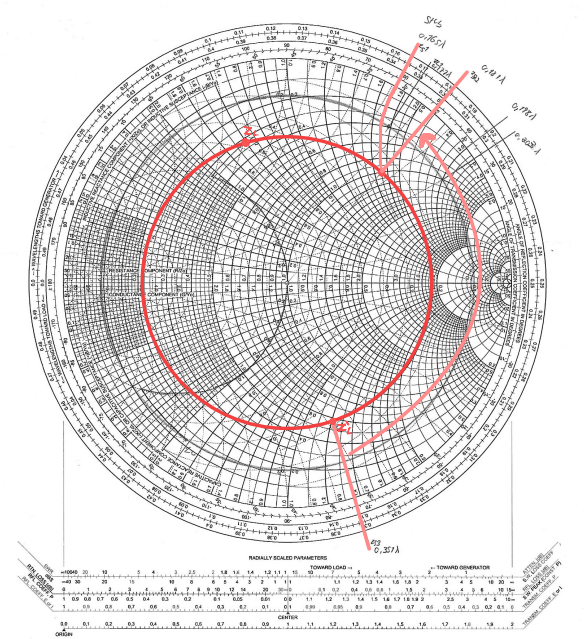
\includegraphics[width=0.65\textwidth]{IMAGENS/CS_LS_ZL.png}
    \caption{Carta de Smith para Linhas e Stubs, $Z_{L}$}
    \label{fig:carta_smith_ls_zl}
\end{figure}


Finalmente vamos adaptar a impedãncia de saída $Z_L = 0.33+j0.70$.

Como dito anteriomente, passamos o valor para admitânica e obtemos o valor $Y_L = 0.55 - j1.17$, com
um comprimento de onda correspondente é $\lambda_{L1} = 0.351~\lambda$

Assim, seguindo até ao ponto de interseção, o valor obtido é $\lambda_{L2} = 0.181~\lambda$. Assim, o valor a colocar na linha
é:
\begin{center}
    $\lambda_{L1} - \lambda_{L2} = 0.351\lambda - 0.181\lambda = 0.170\lambda$
\end{center}

Para o stub, apenas precisamos de ver o valor da parte imaginária desse ponto, que corresponde a $\lambda_{S} = 0.165~\lambda$.

Calculando os atrasos $T_d$ para colocar na análise, obtemos os seguintes valores:
\begin{center}
    $T_{dL} = \frac{0.170}{6~GHz} = 28.33~pS \hspace{3cm} T_{dS} = \frac{0.165}{6~GHz} = 27.50~pS$
\end{center}


% ======== LTspice adaptação: L & S - CIRCUITO ========
\vspace{1cm}
\textbf{Adaptação em LTspice:}
\begin{figure}[H]
    \centering
    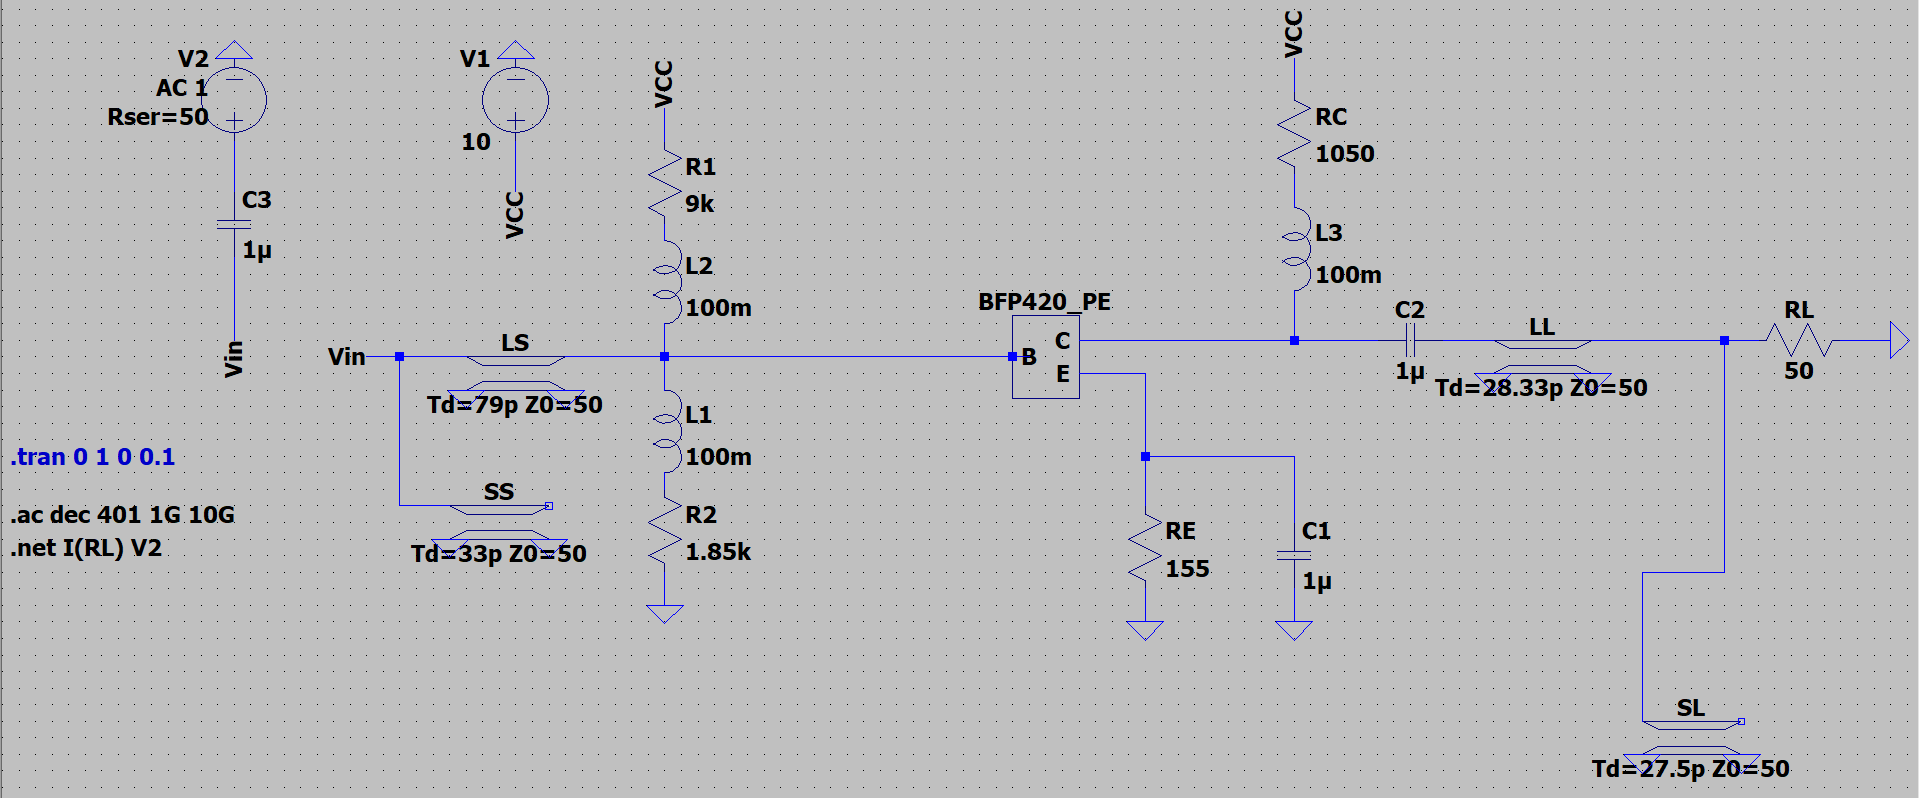
\includegraphics[width=0.8\textwidth]{IMAGENS/ltspice_LS.png}
    \caption{Circuito adaptado com Linhas e Stubs}
    \label{fig:LTspice_LS_circuito}
\end{figure}


\begin{figure}[H]
    \centering
    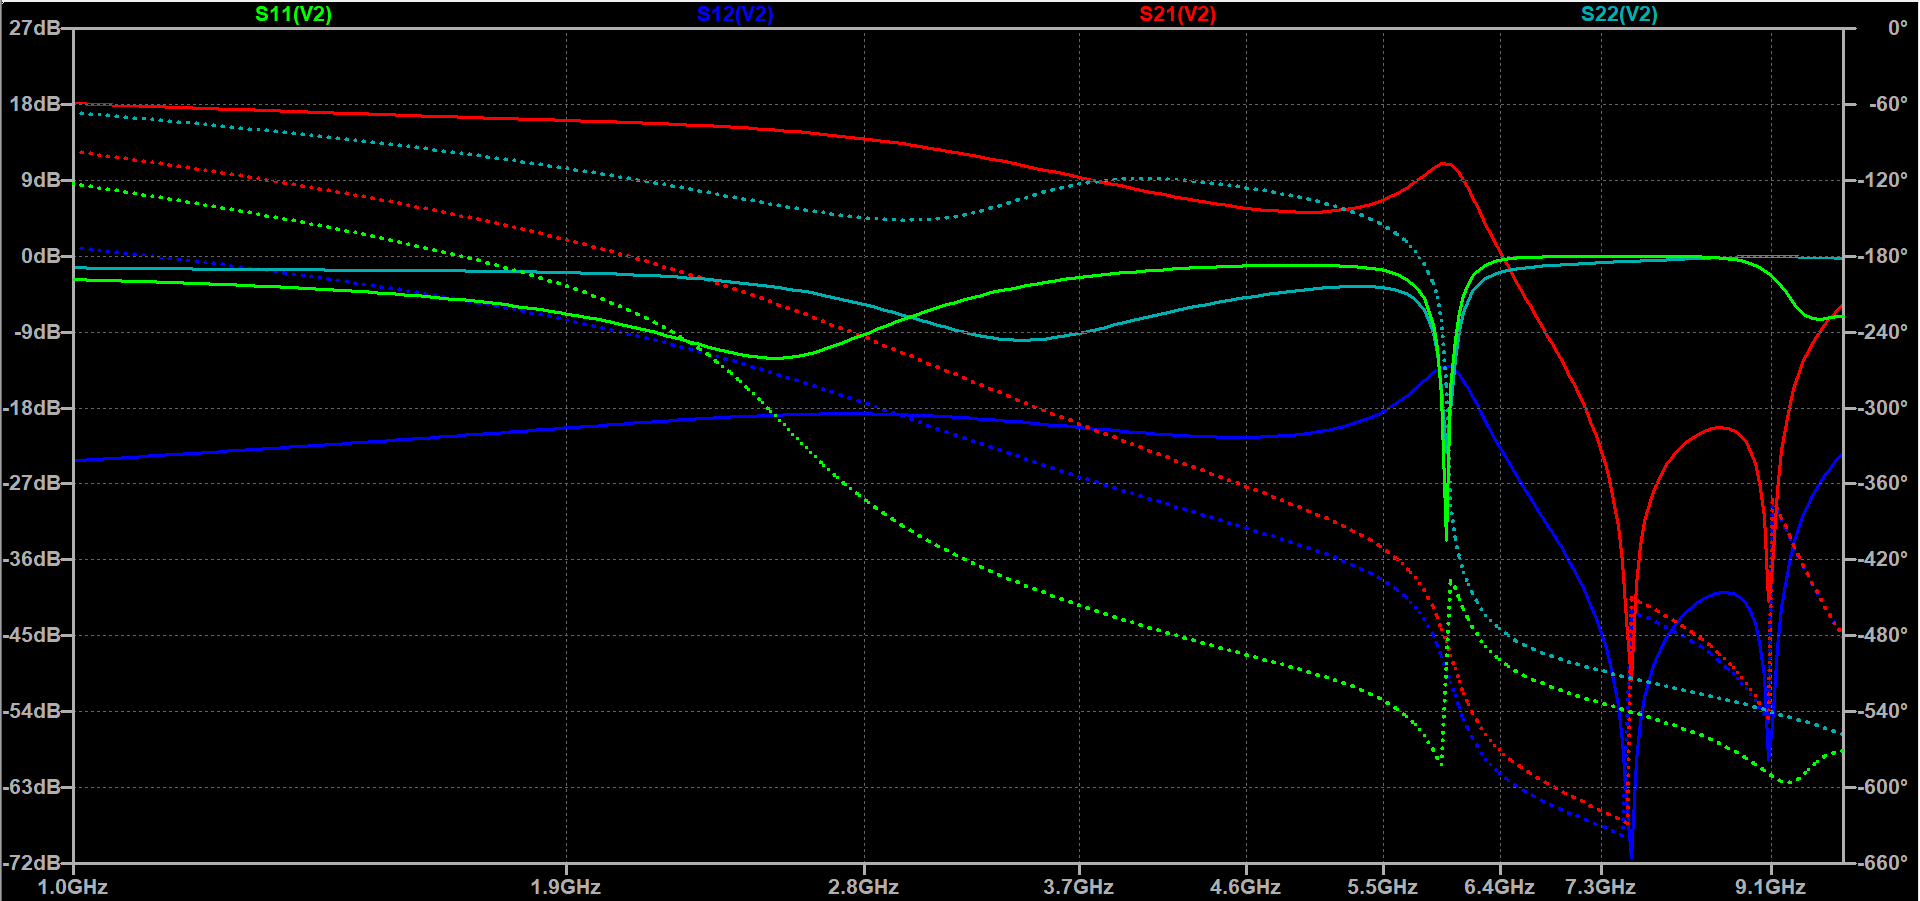
\includegraphics[width=0.8\textwidth]{IMAGENS/ltspice_LS_s.png}
    \caption{Parâmetros S do circuito adaptado com Linhas e Stubs}
    \label{fig:LTspice_LS_s}
\end{figure}

\vspace{0.5cm}
\begin{figure}[htbp]
    \centering
    \begin{subfigure}[b]{0.32\textwidth}
        \centering
        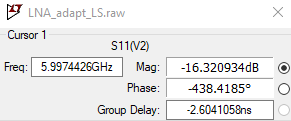
\includegraphics[width=\textwidth]{IMAGENS/ltspice_LS_S11.png}
        \caption{Parâmetro $S_{11}$ (Entrada).}
        \label{fig:s11_ls}
    \end{subfigure}
    \hfill
    \begin{subfigure}[b]{0.32\textwidth}
        \centering
        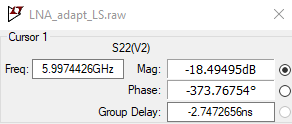
\includegraphics[width=\textwidth]{IMAGENS/ltspice_LS_S22.png}
        \caption{Parâmetro $S_{22}$ (Saída).}
        \label{fig:s22_ls}
    \end{subfigure}
    \hfill
    \begin{subfigure}[b]{0.32\textwidth}
        \centering
        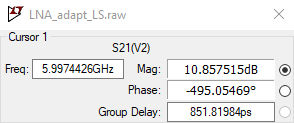
\includegraphics[width=\textwidth]{IMAGENS/ltspice_LS_S21.png}
        \caption{Parâmetro $S_{21}$ (Ganho).}
        \label{fig:s21_ls}
    \end{subfigure}

    \caption{Valores dos parâmetros S do circuito adaptado com Linhas e Stubs}
    \label{fig:valores_s_ls_ltspice}
\end{figure}


Assim, como podemos observar pelas figuras \ref{fig:LTspice_LS_s} e \ref{fig:valores_s_ls_ltspice}, os valores encontram-se
bem adaptados para a frequência esoclhida de $f = 6~GHz$, pois nessa frequência temos $S_{11}$ e $S_{22}$ menores que $-10~dB$ 
($-16.32~dB$ e $-18.49~dB$, respetivamente), enquanto o ganho continua semelhante ao da adaptação com condensadores e bobinas,
sendo este $S_{21} \approx 10.86~dB$



% ======== Cadence ========
\vspace{1cm}
\subsection{Implementação no Cadence e obtenção dos parâmetros S do circuito real}


\vspace{1cm}
% ======== Cadence adaptação ========
\subsection{Adaptação do circuito no Cadence}


\vspace{1cm}
% ======== Cadence adaptação: C & B ========
\subsubsection{Adaptação do circuito no Cadence usando Condensadores e Bobinas}


\vspace{1cm}
% ======== Cadence adaptação: L & S ========
\subsubsection{Adaptação do circuito no Cadence usando Linhas e Stubs}